\chapter{Hardware}
The hardware design is split into several steps in this paper. First, I had to decide if it's really necessary to build a new device or if I can find a suitable solution on the market. When we want to select a suitable device for our task, we have to know the specification of the task itself. The task is specified in section \ref{HWtaskAnalysis}. Based on the task we can specify all requirements that the selected device should meet (section \ref{HWrequirements}). Now, we can start looking for a device that fulfills all the requirements (section \ref{HWavailableSolutions}).

When we don't find any suitable device on the market, we can start to think about creating a new one. In my opinion it's not a good way to start any development before doing the previous steps.

When we already start a development of a new hardware we can think about adding some additional requirements for increasing the versatility of the final hardware. Of course, the new requirements mustn't rapidly increase the final prize. But if the hardware will be used only in the specific task, it's usually unnecessary to add any other functionality. In this case I'm adding some additional requirements in section \ref{HWadditionalRequirements}, because I think that in this case I can add very high versatility with very low additional cost. The analysis of the final expenses is in section \ref{HWadditionalCosts}.

When I'm decided to develop a new hardware and I have the specification of all the requirements, I can start the development process. The selection of chips and other parts is in section \ref{HWdeviceSelection} and the printed circuit board (PCB) design is discussed in section \ref{HWpcbDesign}.

Finally, the manufacturing of the first prototype is described in section \ref{HWmanufacturing}. With the first prototype it's time for testing. The tests should find as many errors as possible and they should proof us if the requirements were already met. The section \ref{HWtesting}. The whole process is shown in the figure \ref{fig:HWprocess}.

\begin{figure}
	\centering
	\label{fig:HWprocess}
	\caption{Flowchart of the hardware design process}
	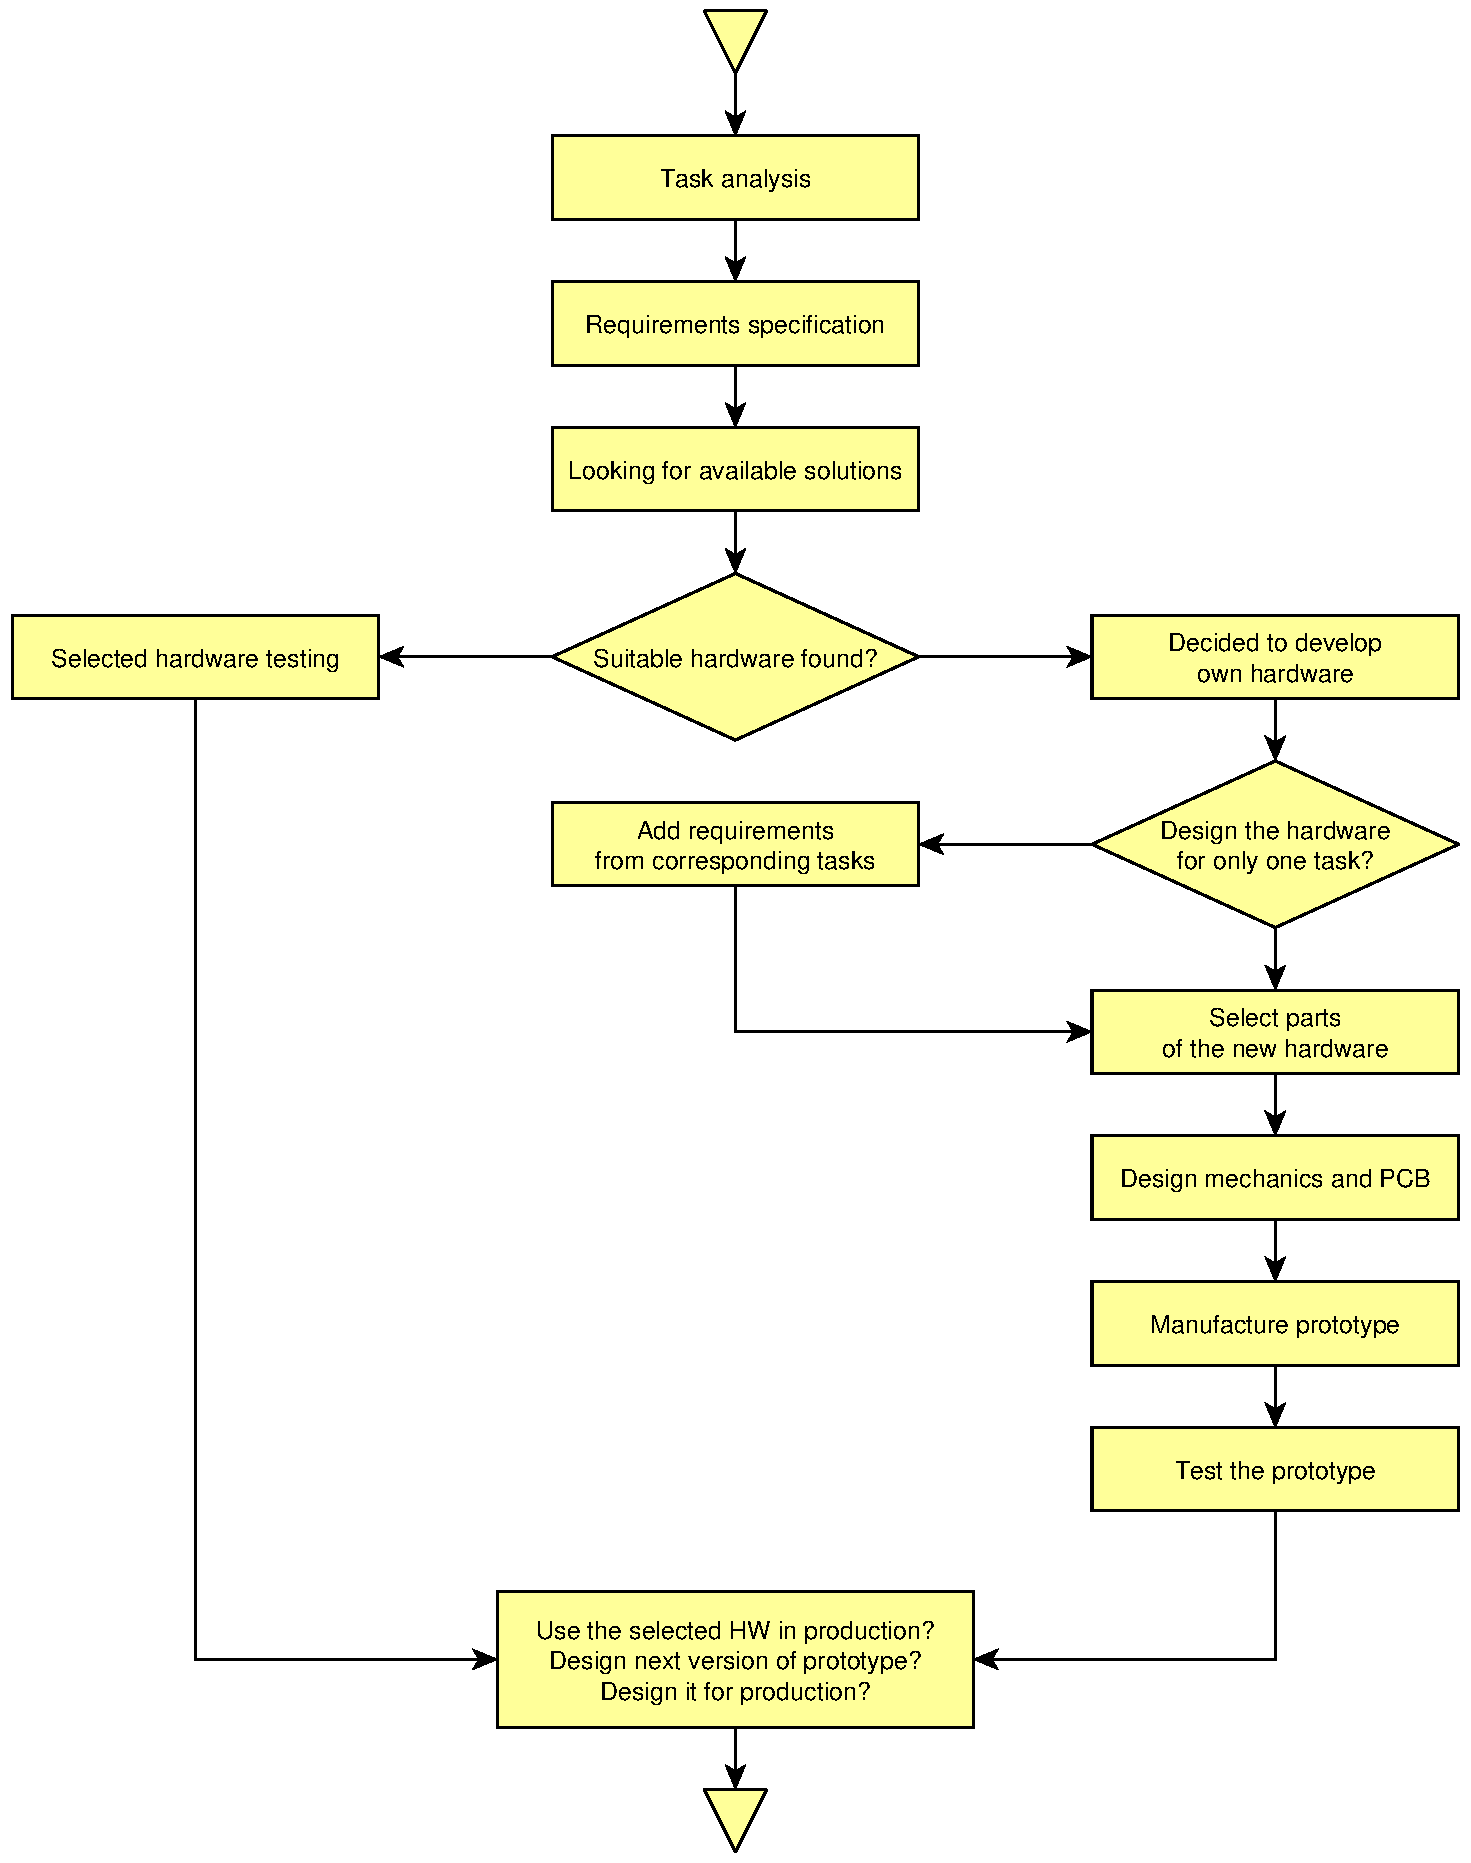
\includegraphics[width=16cm]{../thesis/img/HWdesignProcess.pdf}
\end{figure}

\section{Task Analysis}
\label{HWtaskAnalysis}
When we define our complete task in the first step, then we can derive all requirements for our solution. Finally, we can check if our project was successful based on the previously defined task and requirements.

\highlightedBox{Movement analysis task description}{
	\begin{enumerate}
		\item Measuring of the movement of a subject
		\item Logging the measured data and sending them to post-processing
		\item Analysing of the movement and naming the specific categories of movements
	\end{enumerate}
}

The subject is an animal -- horse in this paper -- or human being or a moving machine. The post-processing can be done real-time during the measurement process, but this is not mandatory. The analysis is primarily focused to recognize known movements in logged data. For example the categories of movement of a horse are: stand, walk, trot, gallop, \dots

\section{Requirements}
\label{HWrequirements}
The development of a new hardware or software is usually driven by specified requirements. In this paper I have specified two groups of requirements. The first group is based on the selected task to solve. The second group has lower priority and specifies all the requirements that I found during other similar tasks with similar hardware. The second group of requirements is adding higher versatility to the final electronic device with very low additional cost. These two groups of requirements are later merged and used as a source for next development of the hardware.

\subsection{High level requirements}

\paragraph{Measuring of the movement of a subject:} The solution should work outdoor. So, we cannot take into account any studio or laboratory based technologies like Motion Capture (Mo-cap). On the other hand we can replace the passive or active markers by whole sensors and remove the necessary cameras. The sensor based electronics is easier to install and can be used in large and complex areas. Based on this outdoor requirement I will consider only wearable sensor systems.

\paragraph{Logging the measured data and sending them to post-processing:} There are no wires acceptable in outdoor use, so we can log the data to internal memory or transmit them via any wireless technology. The wireless systems may be not fully reliable in complex areas with many objects. So, when we want to transmit the data directly it's still better to log them internally for later downloads.

\paragraph{Analysis of the movement and naming the specific categories of movements} This is a software requirement, so it's not very important during the hardware design. But this requirement defines what data we need to measure and this is a hardware requirement.

For the movement reconstruction we need primarily data about position and attitude of every sensor. Some methods for movement classification don't need to know the exact location (for example accelerometer based step counter). This task is focused on developing a new analysis of the movement, so now I cannot exactly say what sensors will be needed in the future. I can make a prediction that the inertial measurement unit (IMU) and some location sensors will be needed. But there are some other sensors that produce interesting data according to the movement analysis, for example a heart rate sensor according to animals.

Finally, I would like to add as many interesting sensors as possible, because it will give us more data sources and we are less limited by the data sources. The other advantage is multifunctionality of the hardware. On the other hand these additional sensors should be added only into additional requirements with lower importance. Otherwise the selection of an appropriate hardware (based on the requirements) will be manipulated by number of probably unnecessary sensors.

\subsection{Low level requirements}
Finally, I've chosen a wearable sensors technology. The next requirements are specific to this technology and focused on selection of the devices. Let's call a used wearable device or devices as Sensor Board. The table \ref{tab:requirements} shows the list of requirements for this Sensor Board.

\begin{table}
\centering
\caption{Sensor Board low level requirements 1}
\label{tab:requirements}
\begin{tcolorbox}[tab2,tabularx={X|p{10cm}},title=Importance legend]
	\greenLow	& Nice to have \\
	\yellowMedium & Very useful, reduce time or human effort \\
	\redHigh & Mandatory, impossible without this functionality \\
\end{tcolorbox}
\vspace{1cm}
\begin{tcolorbox}[tab2,tabularx={|c|X|c|l|},title=Low level requirements 1]
	Category & Requirement & Importance & Comment \\ \hline \hline
	
	& Accumulator & \redHigh &  \\
	& Battery percentage indicator & \redHigh &  \\
	& Charging when external power applied & \redHigh &  \\
	& Voltage and current sensor & \yellowMedium &  \\
	& Power LED & \redHigh &  \\
	& Power switch & \redHigh &  \\
	& Automatic selection between external and battery power & \redHigh &  \\
	\multirow{-8}{*}{Power Supply} & Standardized charging connector & \yellowMedium &  \\ \hline
	
	& Accelerometer & \redHigh &  \\
	& Dynamic Gyroscope & \redHigh &  \\
	& Magnetometer & \redHigh &  \\
	& Indoor position & \yellowMedium &  \\
	& Outdoor position & \greenLow &  \\
	& Barometer & \greenLow &  \\
	\multirow{-7}{*}{Sensors} & Board temperature & \greenLow &  \\ \hline
	
	& Allow user programming & \redHigh &  \\
	& Wireless programming & \greenLow &  \\
	& Wired programming & \redHigh &  \\
	& Wireless & \redHigh &  \\
	& Standardized protocol & \redHigh &  \\
	& Wired access & \redHigh &  \\
	\multirow{-7}{*}{Communication} & Connector for external sensors & \greenLow &  \\ \hline
\end{tcolorbox}
\end{table}

\begin{table}[H]
	\centering
	\caption{Sensor Board low level requirements 2}
	\label{tab:requirements}
	\begin{tcolorbox}[tab2,tabularx={|c|X|c|l|},title=Low level requirements 2]
		Category & Requirement & Importance & Comment \\ \hline \hline
		
		& Logging all data for several hours & \redHigh &  \\
		& Sensor fusion coprocessor & \greenLow &  \\
		\multirow{-3}{*}{Functions} & LED indicators & \redHigh &  \\ \hline
		
		& Wearable design & \redHigh &  \\
		& Dimensions under \SI{6}{cm} & \redHigh &  \\
		& Dimensions under \SI{3}{cm} & \greenLow &  \\
		& Weight under \SI{50}{g} & \redHigh &  \\
		\multirow{-5}{*}{Mechanical} & Weight under \SI{20}{g} & \greenLow &  \\ \hline
		
		& Control multiple devices simultaneously & \yellowMedium &  \\
		& Download logged data & \redHigh &  \\
		& Streaming data during measurement & \yellowMedium &  \\
		& Start logging on multiple devices by clicking one button & \yellowMedium &  \\
		& Time synchronization of multiple devices & \redHigh &  \\
		\multirow{-6}{*}{Software} & Possibility to upload data to a server & \redHigh &  \\ 
	\end{tcolorbox}
\end{table}

\subsection{Additional requirements}
\label{HWadditionalRequirements}
The additional requirements are shown in table \ref{tab:additionalReq}.

\begin{table}[H]
\centering
\label{tab:additionalReq}
\caption{Sensor Board additional requirements 2}
\begin{tabular}{|c|p{10cm}|}
	\hline
	\multicolumn{2}{|c|}{Importance} \\ \hline \hline
	\greenLow	& Nice to have \\ \hline
	\yellowMedium & Useful, can significantly improve functionality \\ \hline
	\st{\redHigh} & Not applicable \\ \hline
\end{tabular}
\newline
\vspace{1cm}
\newline
\begin{tabular}{|c|p{5cm}|c|l|}
\hline
Category & Requirement & Importance & Comment \\ \hline
Functions & Coprocessor for periodic computations like sensor fusion & \greenLow &  \\ \hline
Functions & Piezo buzzer & \greenLow &  \\ \hline
Functions & Buttons & \yellowMedium &  \\ \hline

Sensors & Ambient light & \greenLow &  \\ \hline
Sensors & Humidity & \greenLow &  \\ \hline
Sensors & Sound (microphone) & \greenLow &  \\ \hline
Sensors & Ambient temperature & \greenLow &  \\ \hline

Communication & UART, I2C, SPI connector & \greenLow &  \\ \hline
Communication & PWM outputs & \greenLow &  \\ \hline
Communication & Analog inputs & \greenLow &  \\ \hline

Software & NMEA input & \greenLow &  \\ \hline
\end{tabular}
\end{table}

\section{Available solutions}
\label{HWavailableSolutions}
The table \ref{tab:availableSolutions} shows the overview of existing devices I have found.

\begin{table}[H]
\centering
\caption{Available solutions}
\label{tab:availableSolutions}
\begin{tabular}{|l|l|l|l|l|l|}
\hline
       & & & \multicolumn{3}{|c|}{Number of unfullfilled requirements} \\
Device & Datasheet & Price & Low & Medium & High \\\hline\hline

MetaWear &  &  &  &  &  \\
ArduPilot 2.6 &  &  &  &  &  \\
X-IMU &  &  &  &  &  \\
wearable... &  &  &  &  &  \\\hline
\end{tabular}
\end{table}

\section{Selection of devices}
\label{HWdeviceSelection}
//todo



\section{PCB design}
\label{HWpcbDesign}
The PCB design should meet both electrical and mechanical requirements. It's usually easier to design a large board in the first iteration, which is used only in the laboratory for software development and testing. Then the second iteration brings the first practically usable device and probably the third iteration is the first one dedicated for production use.

Here in this process I will merge the first and the second version together. I will create a larger device which is still usable as wearable device. This implies that I can do the software development, laboratory tests and the first outdoor tests with the same board designed during the first iteration. I'm going to decrease the dimensions of the first prototype by splitting the PCB to separate sandwich modules. The testing process should give us advantages and disadvantages of this mechanical solution.

I have used CadSoft EAGLE (Easy Applicable Graphical Layout Editor) \cite{EAGLE} during this process. I've finally chosen this editor because it has the availability of the libraries for the devices I wanted to use. I would probably use KiCad \cite{KiCad} if there was the same availability of the libraries.

\subsection{Schematics and board layout}
The schematics and the board layout was created in CadSoft EAGLE \cite{EAGLE}. The figures \ref{sch1} and \ref{sch2} shows the exported schematics split into two sheets. The exported PCB layout drawing in scale 1:1 is in figure \ref{brd1} and in scale 2:1 with more details in figure \ref{brd2}.

\begin{figure}[H]
	\centering
	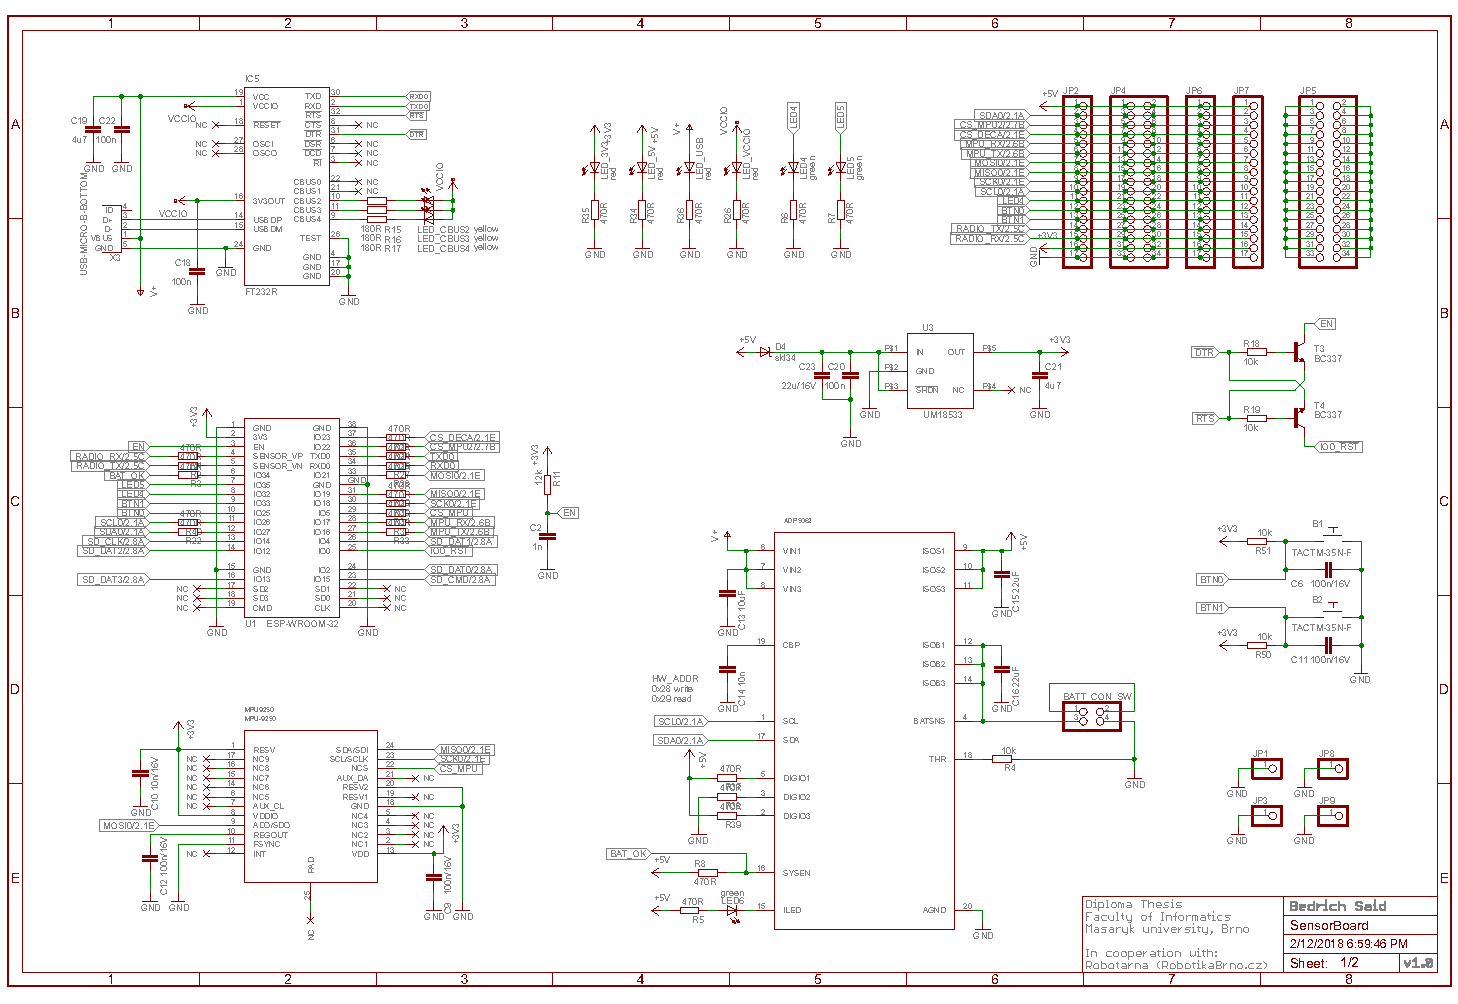
\includegraphics[angle=90, scale=1]{img/sch1.pdf}
	\label{sch1}
	\caption{Schematics of the Sensor Board sheet 1}
\end{figure}

\begin{figure}[H]
	\centering
	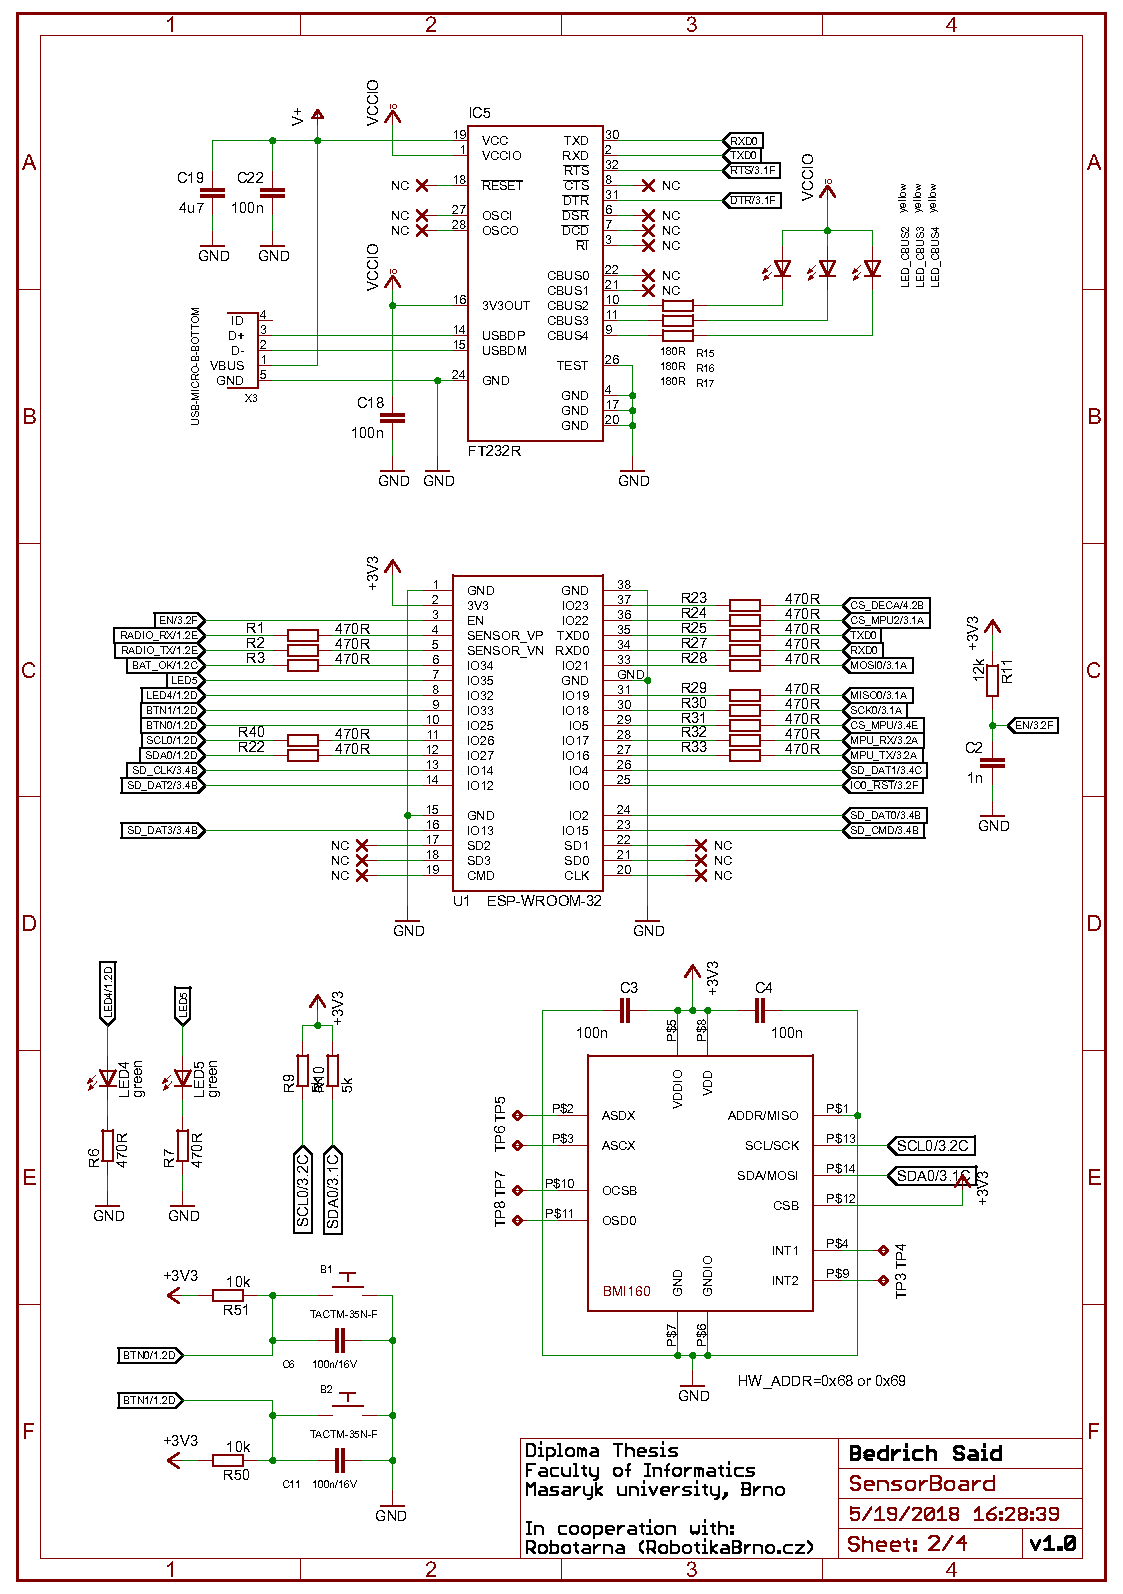
\includegraphics[angle=90, scale=1]{img/sch2.pdf}
	\label{sch2}
	\caption{Schematics of the Sensor Board sheet 2}
\end{figure}

\begin{figure}[H]
	\centering
	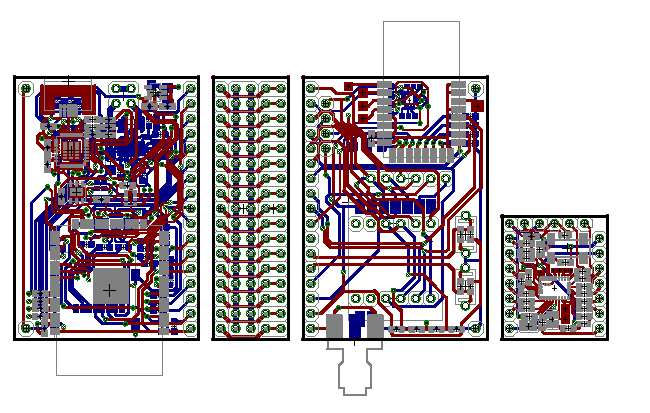
\includegraphics[scale=1]{img/brd.pdf}
	\begin{center}
		Top and Bottom layer
	\end{center}
	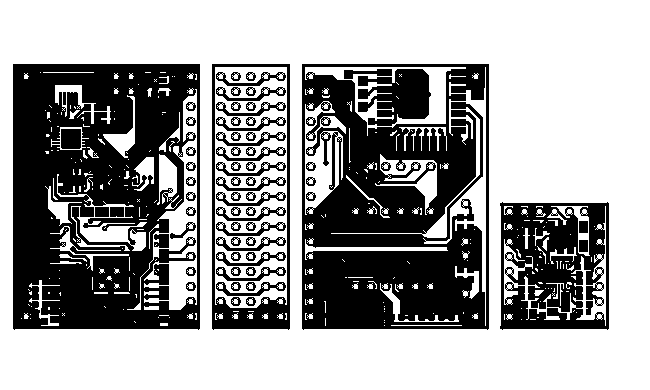
\includegraphics[scale=1]{img/brdTop.pdf}
	\begin{center}
		Only Top layer
	\end{center}
	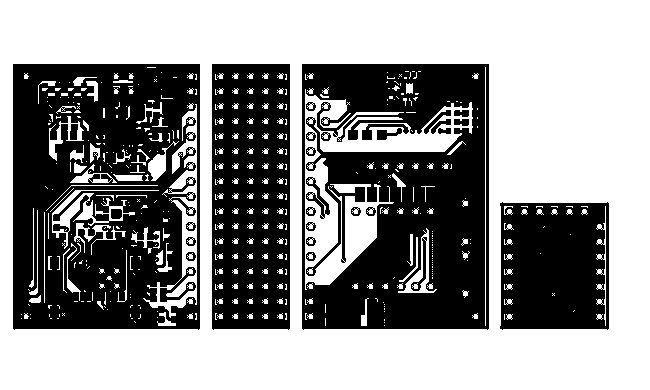
\includegraphics[scale=1]{img/brdBottom.pdf}
	\begin{center}
		Only Bottom layer
	\end{center}
	\label{brd1}
	\caption{Sensor Board layout in scale 1:1}
\end{figure}

\begin{figure}[H]
	\centering
	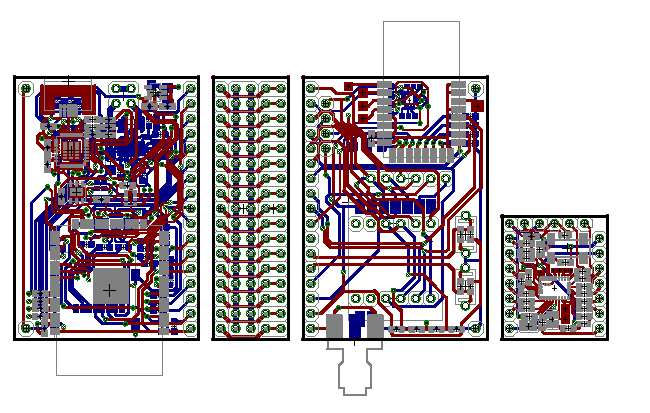
\includegraphics[angle=90, scale=2]{img/brd.pdf}
	\label{brd2}
	\caption{Sensor Board layout in detail scale 2:1}
\end{figure}

\subsection{Mechanical layout and connectors}
The mechanical layout is shown in figure \ref{fig:HWdimensions}.

\begin{figure}[H]
	\centering
	\label{fig:HWdimensions}
	\caption{Sensor Board dimensions}
	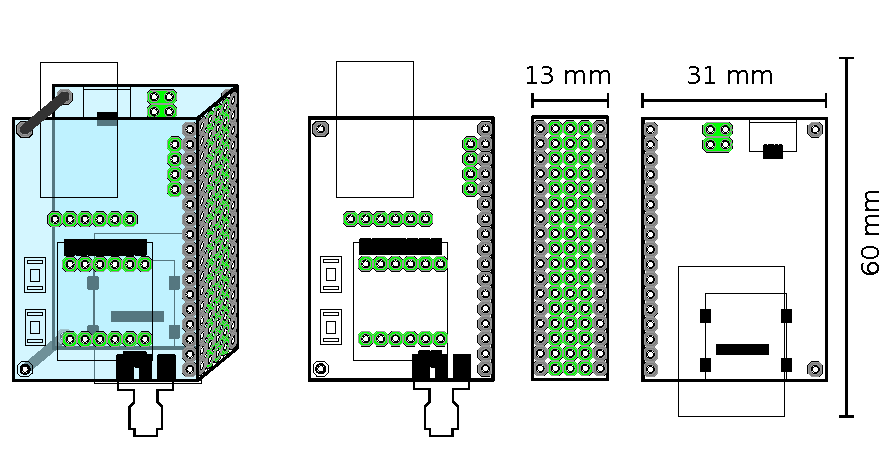
\includegraphics[scale=1]{img/HWdimensions.pdf}
\end{figure}

\section{Manufacturing}
\label{HWmanufacturing}
//todo: pridat vsude fotky jednotlivych fazi

The manufacturing process of the prototype consists of these steps:
\begin{enumerate}
	\item Collecting source data -- schematics and board layout (in this paper in Eagle)
	\item Manufacturing of the Printed Circuit Board (PCB)
	\begin{enumerate}
		\item Panelization of the board layout
		\item Adding calibration markers
		\item Export gerber files
		\item Send exported files to manufacturing company
	\end{enumerate}
	\item Machine surface mount technology (SMT)
	\begin{enumerate}
		\item Export data for template for applying solder paste
		\item Export partlist -- list of all devices with their coordinates
		\item Export bill of materials (BOM)
		\item Manufacturing of the template for applying solder paste
		\item Order all devices according to BOM
		\item Sending template for applying solder paste, packages with devices and partlist to the manufacturer
	\end{enumerate}
	\item Finalization of the prototype
	\begin{enumerate}
		\item Hand soldering of some remaining devices like connectors or wires
		\item Completing the final prototype from possible parts and packaging
		\item Applying power and first testing
	\end{enumerate}
\end{enumerate}

\subsection{Collecting source data}
The source data may be in various formats according to the used tools. I used CadSoft EAGLE \cite{EAGLE} during the development, but many other tools are available on the market. It depends on the manufacturer company if they accept the source data in our format. They usually accept the source data, but they usually apply an exporting fee. All PCB editors should be able to export the manufacturing data in standardized formats. (Sometimes it's very hard or impossible to edit the exported data.)

\subsection{Manufacturing of the Printed Circuit Board}
When we have more than one board we should assemble all boards onto one or more panels. If we plan to solder the devices by machine we should add a calibration marks on the final panel. I have followed the instructions from SMTplus company \cite{SMTplusManual}.

First, I have panelized the seprated boards and I have added the calibration marks according to the rules of SMTPlus company \cite{SMTPlusDesignRules}. Finally, I have exported the gerber files using a CAM job \cite{GatemaCAMjob} in Eagle. I have followed the design rules for class 3 by Gatema a.s. company \cite{GatemaDesignRules}.

\subsection{Machine surface mount technology}
We need the PCB, template for soldering paste and all devices in this step. Some PCB manufacturers offer creating the template as well, so this is the way I used. The thickness of the template indicates the volume of the paste on each pad. For my small SMDs I used \SI{100}{\micro\meter}, but I recommend to discuss the parameters with the manufacturer.

The BOM and partlist export depends on the used design tools. When we connect used devices in the sources directly with their part numbers on selected shops, we can simply export the partlist and then import it on the seller's website. I recommend to buy some spare devices to minimize the risk of their damage.

\begin{figure}[H]
	\centering
	\label{smtPasteTemplate}
	\caption{Template for soldering paste in scale 1:2}
	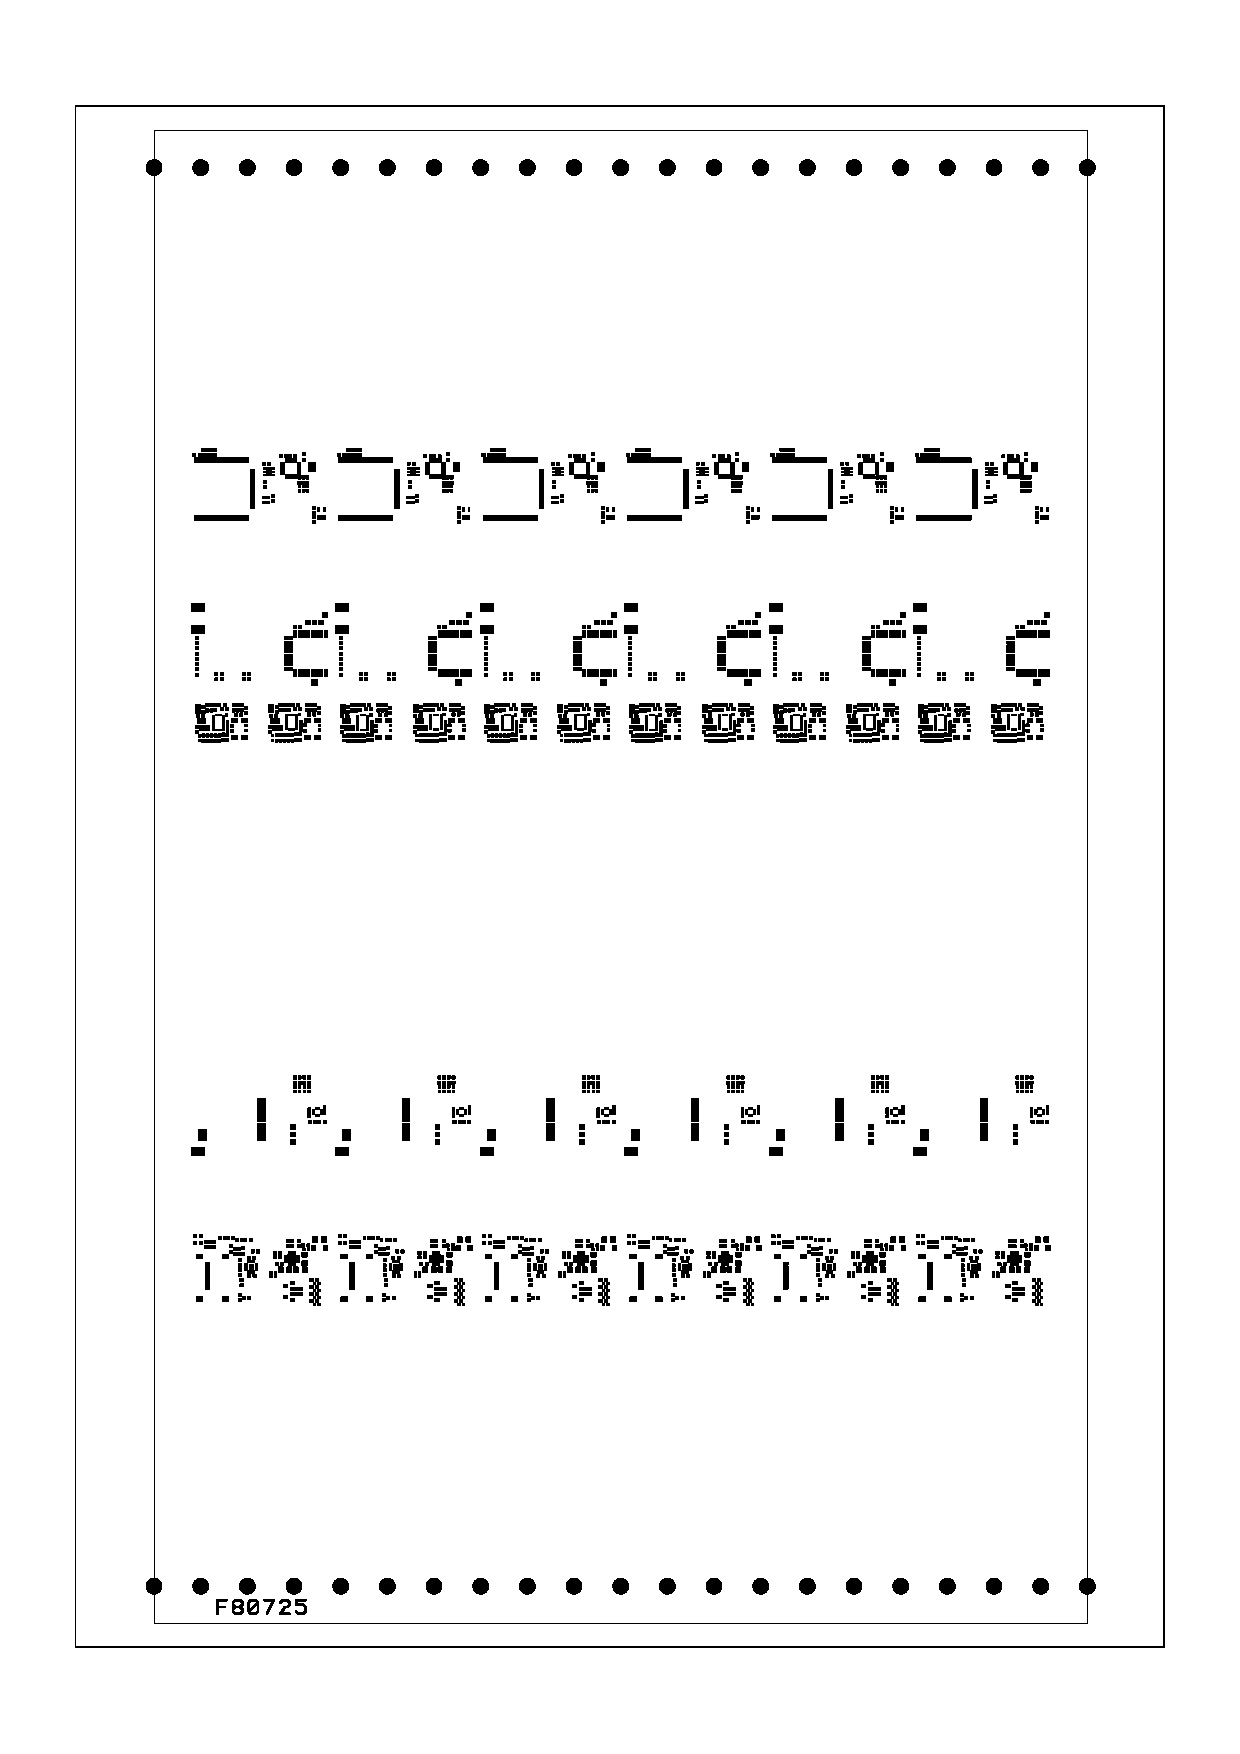
\includegraphics[angle=90, scale=0.5]{img/smtPasteTemplate.pdf}
\end{figure}

\subsection{Finalization of the prototype}
We can discuss the finalization work with the manufacturer, but when we create a prototype, I have to recommend to do this job by ourself. It allows us to perform some tests before packaging and we don't have to spend time and money with preparation of the documentation about how to assemble and package our prototype. Otherwise the different software developers and testers can receive the different parts of the prototype for their next work.

\section{Testing}
\label{HWtesting}
The testing process has been split into two parts: the laboratory testing during the software development and the outdoor testing. I have found some errors in the version 1.0 during the laboratory testing. These errors are described in Errata list in section \ref{errata}. I did another tests against the specification of used devices. The results show us what devices should be used in the next version of the hardware and what devices are redundant. The results are shown in the section \ref{deviceTesting}. The outdoor tests didn't find any significant errors, but there were found several recommendations for the future versions of the Sensor Board. These recommendations are mentioned in section \ref{recommendationsNextVerison}.

\subsection{Errata}
\label{errata}
The table \ref{errataTable} shows all errors I have found during software development and laboratory testing of the Sensor Board prototype.

\begin{table}[H]
\centering
\caption{Errata of the Sensor Board}
\label{errataTable}
\begin{tabular}{|l|l|}
	\hline
	\multicolumn{2}{|l|}{Severities} \\ \hline
	\greenLow & No significant affects \\ \hline
	\greenSpare & Only spare devices may not work \\ \hline
	\yellowMedium & Some part of the prototype may not work \\ \hline
	\redHigh & The prototype has to be remade \\ \hline
\end{tabular}
\begin{tabular}{|c|p{6cm}|p{2.5cm}|c|c|}
\hline
Number & Description & Error created during & Image & Severity \\ \hline
1      &
	\parbox{6 cm}{Bridge between boards under micro USB connector\\ \\ What happens:\\ The micro USB connector may be placed with lower accuracy}
	& panelization         &       & \greenLow      \\ \hline
	
2      &
	\parbox{6 cm}{Swapped MISO and MOSI on pins IO19 and IO21 on the ESP-WROOM-32 chip according to ESP32 Arduino standard\\ \\ What happens:\\ The SPI interface is not working in Arduino compatible mode without modification of the Arduino SPI library}
	& schematics design    &       & \yellowMedium   \\ \hline
	
3      &
	\parbox{6 cm}{LED5 connected to IO35 on ESP-WROOM-32 is not working\\ \\ What happens:\\ The pins IO34 -- IO39 are input only, so they cannot drive a LED}
	& schematics design    &       & \greenSpare    \\ \hline
	
4      &
	\parbox{6 cm}{Missing pull-up resistors on SD card\\ \\ What happens:\\ The SDIO interface needs external pull-up resistors to work properly. I have added these resistors later by hand.}
	& schematics design    &       & \yellowMedium   \\ \hline
	
5      &
	\parbox{6 cm}{The temperature measurement is placed very close to the main processor\\ \\ What happens:\\ The processor heating affects the measured temperature}
	& board layout         &       & \greenSpare    \\ \hline
	
6      &
	\parbox{6 cm}{Low capacity capacitor placed on power supply\\ \\ What happens:\\ When we use WiFi some brownouts can be detected. I have added a bigger capacitor later by hand.}
	& schematics design    &       & \yellowMedium   \\ \hline
	
7      &
	\parbox{6 cm}{The light sensor is placed on inner side of the board\\ \\ What happens:\\ The measured values are affected by shadow of the board}
	& board layout         &       & \greenSpare    \\ \hline
8      &
\parbox{6 cm}{Missing safety resistors on pins with buttons. These pins are directly connected to processor.\\ \\ What happens:\\ When the pins are defined in software to be used in different way, incorrect connection can burn the processor. }
& schematics design        &       & \yellowMedium   \\ \hline
\end{tabular}
\end{table}

\subsection{Device testing}
\label{deviceTesting}
The device testing may select the devices used in the future versions and remove all spare parts from the prototype. The table \ref{deviceTestsTable} shows the test results and the table \ref{deviceSelectionTable} shows the devices that I recommend to use in future versions.

\begin{table}[H]
\centering
\caption{Device tests}
\label{deviceTestsTable}
\begin{tabular}{|l|l|l|}
	Device & Test & Result \\
	MPU9250 & SPI interface & Warning \\
	MPU9250 & I2C interface & Pass    \\
	//todo & ... & ... \\
\end{tabular}
\end{table}

\begin{table}[H]
\centering
\caption{Device selection}
\label{deviceSelectionTable}
\begin{tabular}{|l|l|}
	\hline
	\multicolumn{2}{|l|}{Decision} \\ \hline
	Selected & recommended for use in future versions \\ \hline
	Possible & Not necessary, but has use-cases \\ \hline
	Removed & Not recommended or will be spare \\ \hline
\end{tabular}
\begin{tabular}{|l|l|l|}
	\hline
	Device & Decision \\ \hline
	MPU9250 & Removed \\ \hline
	BMF055 & Selected \\ \hline
	//todo & ... & ... \\ \hline
\end{tabular}
\end{table}

\subsection{Recommendations for the next version}
\label{recommendationsNextVerison}
Recommendations for the future versions of the Sensor Board based on the outdoor testing:
\begin{itemize}
	\item[--] Replace software LEDs by one or more RGB LEDs. For example WS2812 RGB LED \cite{AdafruitLED}.
	\item[--] Move the sensor fusion and computations to Atmel SAM D21 \cite{AtmelSAM} processor inside the BMF055 \cite{BMF055} chip. Keep the ESP32 \cite{ESP32} processor only for communication and user computations.
	\item[--] Decrease board dimensions using 4 layer PCB. The increased cost for 4 layer board may be saved on smaller surface.
	\item[--] Sometimes it is better to have all SMDs at one side of the board. The manufacturing is cheaper and the space on the second side can be used for example for battery mounting or for connectors.
	\item[--] Split the board area to an area for sensors, an area for power electronics and an area for computing. The power distribution is easier in this situation and the sensors are less influenced by other electronics.
	\item[--] Use another driver with more capabilities for USB connection. The USB on board actually supports only UART communication on virtual COM port. The File Transfer protocol for the SD card should be supported, too. (If it is needed we can add full USB host support or USB-C compatibility.)
	\item[--] Add specialized pads for oscilloscope. The pads are connected to the signal and to the ground, so the oscilloscope measurements are more accurate.
	\item[--] The main processor should be able to switch on/off the power of other parts (sensors). The sensors support sleep modes, but we cannot completely switch them off to save more energy from battery.
\end{itemize}

//todo: pridat informaci o ALB32-WROVER
	
\subsection{Analysis of additional costs}
\label{HWadditionalCosts}
//todo

//todo: citovat vetsi verzi ESP WROOM 32 a vypsat vyhody
